\def\year{2019}\relax
%File: formatting-instruction.tex
\documentclass[letterpaper]{article} %DO NOT CHANGE THIS
\usepackage{aaai19}  %Required
\usepackage{times}  %Required
\usepackage{helvet}  %Required
\usepackage{courier}  %Required
\usepackage{url}  %Required
\usepackage{graphicx}  %Required
\frenchspacing  %Required
%\usepackage{biblatex}
\usepackage{comment}
\usepackage{cleveref}
\usepackage{amssymb}
\usepackage[
backend=biber,
style=alphabetic,
sorting=ynt
]{biblatex}
\addbibresource{sample.bib}

\setlength{\pdfpagewidth}{8.5in}  %Required
\setlength{\pdfpageheight}{11in}  %Required
%PDF Info Is Required:
  \pdfinfo{}
\setcounter{secnumdepth}{0}  
 \begin{document}
% The file aaai.sty is the style file for AAAI Press 
% proceedings, working notes, and technical reports.
%
\title{Fall 2018 CS7180 Final Project Report}
\author{Peter Bernstein and Giorgio Severi}
\maketitle
\begin{abstract}
As a final project for a Reinforcement Learning course, we construct two distinct learning agents for the 1993 game Doom that learn solely from raw visual information in the game. One solver uses deep Q-learning, which was recently employed with great success in solving various games. The other solver uses SARSA, a tabular method for on-policy temporal difference learning that we consider as a representative baseline of the classical reinforcement learning methods. We show that SARSA makes steady progress toward approximating an optimal policy but within a reasonable time frame it only achieves poor average returns, as expected due to the complexity of the problem. We were unfortunately unable to show meaningful learning results from the DQN agent. This is likely because of the lack of sufficient time to perform training on the available hardware resources.
\end{abstract}

\section{Introduction}
\begin{figure*}[h]
  \centering
  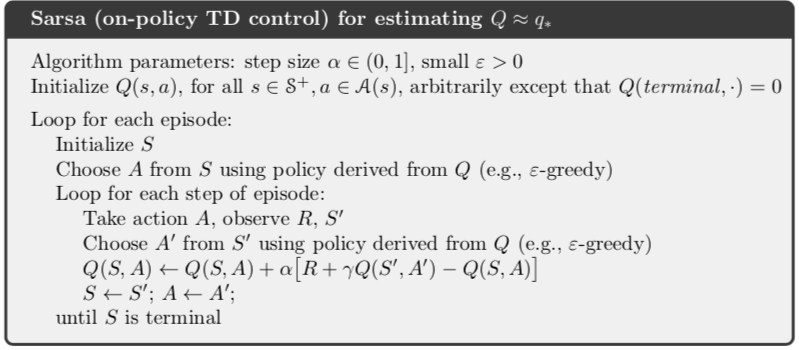
\includegraphics[width = 0.8 \textwidth]{sarsa_algo}
  \caption{High level pseudocode description of SARSA algorithm for estimating $Q$. Figure taken from \cite{sutton_barto}}
  \label{sarsa}
\end{figure*}
Doom is a classic First-Person Shooter (FPS) game from 1993 created by Id Software. As one of the first FPS games to market, it is simple in its gameplay in comparison to contemporary video games, but can still be significantly more complex than many other Atari games, such as Pong, and other toy scenarios from OpenAI Gym, such as Frozen Lake. In Doom, the player is a marine in the central point of an invasion of demons. The agent can be placed in a variety of scenarios with a multitude of differently behaving demons. At any time the agent can navigate, in order to explore the map or pick up ammunition and health packs, or shoot his weapon. The game state may not be completely visible at all times and obstacles often partially obscure the display. 

The above features make Doom an interesting study for reinforcement learning because of the abundance of settings with varying difficulties. Due to the lack of time and access to powerful computational resources, the focus of this project is restricted to a simple game scenario. Given access to more advanced resources, the parameters in this project can easily be changed to train our models on a complex Doom environment.

For our work we employed the ViZDoom \cite{vizdoom} research platform, based on the famous ZDoom\footnote{\url{https://github.com/rheit/zdoom}} open source Doom emulator project. We consider ViZDoom particularly interesting for its vast customizability, and for the large interest shown by the community, which has brought to the organization of an annual ViZDoom competition, where RL bots are pit against each other in a deathmatch scenario.\footnote{\url{http://vizdoom.cs.put.edu.pl/competition-cig-2018}} As implied by the name, ViZDoom allows users to easily access the raw graphical output of the game engine, that was crucial for our project, since we aimed to only make use of visual inputs when training our agents.



\section{Background}
The problem we aim to solve in creating an agent to play a game is the problem of estimating a state-action value function, $Q$, for an environment. In our Doom game, the state of the game is defined by the graphical frame rendered by the game in each time step. The agent has a number of available actions given the state of the game. In our experiments, the available actions to the agent are \texttt{move left}, \texttt{move right}, or \texttt{shoot}. The decision problem that the agent has to solve is which action can he pick to maximize the expected future reward. A function $\pi$ that takes the state of the game and returns an action for the agent to take is called a policy. A policy which correctly selects the best available move to the agent at each time step in order to maximize the expected future reward is called an optimal policy. 

In order to solve this sequential decision problem we can learn estimates for the optimal value of each action, defined as the expected sum of future rewards when taking that action and following the optimal policy thereafter. Under a given policy $\pi$, the true value of an action $a$ in a state $s$ is
$$ Q_{\pi}(s,a) := \mathbb{E}[R_1+\gamma R_2 + ... | S_0 = s, A_0 = a, \pi ], $$ 
where $\gamma \in [0, 1]$ is a discount factor that trades off the importance of immediate and later rewards, and $Q_{\pi}(s,a)$ is the function returning the value of performing the action $a$, given the current state $s$, and then continue following the policy $\pi$. The optimal value is then $Q_*(s,a) = \max_{\pi} Q_{\pi}(s,a)$. An optimal policy is easily determined by selecting the highest valued action in each state once the optimal values are known. 

Our project employs two forms of Temporal-difference (TD) learning, which is a combination of Monte Carlo and dynamic programming techniques to solve a Markov decision process (MDP). In TD prediction of the value function is updated at every time step, rather than at every episode as in Monte Carlo methods. We choose to use SARSA and deep Q-learning (see project description section for more details) due to their wide use in literature.


\begin{figure}[h]
  \includegraphics[width = \columnwidth]{Report/DQN_algorithm.png}
  \caption{Pseudocode description of deep Q-network with memory replay from \cite{mnih2015human}. }
  \label{dqn_algo}
\end{figure}

\section{Related Work}
Reinforcement learning and deep reinforcement learning in particular have a history of success on fully observable games for Atari, such as Pong or Space Invaders \cite{playing_atari}. Most of the best performing AI solvers were trained using deep recurrent Q-learning, weighted replay, or dueling. Google DeepMind recently developed an Asynchronous Advantage Actor-Critic (A3C) model that has also been used to train AI solvers for Atari games with success as well \cite{deepmind}. The victory of AlphaGo over the best human player received wide media attention as a landmark. While we restrict our focus in this project to deep-Q learning and SARSA, more complicated models have proven to be more successful especially running on more advanced architectures. 

Doom in particular has a history with using deep-Q networks to train solvers. Recent works on training the Doom AI have created models that obtain very good performance even in complex, partially observable scenarios with multiple actors \cite{lample}. 

The state of the art of game-playing agents is represented by the OpenAI Five\footnote{\url{https://blog.openai.com/openai-five/}}. This year, in fact, the OpenAI team was able to develop and train a set of five bots that was capable of cooperatively playing the famous Dota 2 game\footnote{\url{http://blog.dota2.com/}}, and beat a team of five retired professional players \cite{openaifive}. This represents a landmark achievement in the field due to both the sheer complexity of the game mechanics and the level of interaction required from the agents.  


\section{Project Description}
We chose a basic scenario of the Doom game to train our agent. The setting for our project places the agent on one side of a square room, and a demon is placed on the opposite side of the room in a random initial position. The agent is allowed to chose one of three actions at any time step: move left, move right, or shoot. For the agent to kill a monster, it must be facing the demon and perform the shooting action. Once placed, the demon is stationary  and does not attack the agent. 

The goal of the agent is to shoot the demon, which will result in the game ending and the agent receiving a reward of $+100$. The agent has a limited amount of ammunition and will receive a negative reward of $-6$ for each wasted shot. If the agent is unable to kill the enemy, the episode will still end after $300$ frames and, for each frame in which the agent is alive, it will receive a negative reward of $-1$ as an incentive to eliminate the enemy faster.

In this project we decided to compare two widely used Reinforcement Learning techniques, both of which are forms of TD learning. The first, SARSA, is based on tabular learning and deep Q-learning is based on deep learning, DQN. These two models were chosen for their vast usage in the RL literature, and the good performances shown while solving other problems.


\subsection{Pre-processing}

\begin{figure}
  \includegraphics[width = \columnwidth]{preproc_orig}
  \caption{A frame of the game during action as rendered by the emulator.}
\label{preproc_orig}
\end{figure}

\begin{figure}
  \includegraphics[width = \columnwidth]{preproc_fin}
  \caption{A processed frame.}
\label{preproc_fin}
\end{figure}

Given our aim to only make use of visual information for the training of our agents, we needed to pre-process the input images rendered by the emulator. We decided to perform the following pre-processing steps:
\begin{itemize}
    \item conversion to gray-scale; \footnote{We note here that the default method used in most projects to achieve RGB to gray-scale conversion is through the scikit-image library. We note, however, that this method is noticeably slower than a direct manipulation of the image array through numpy functions. This is due to the employment of a method which should improve the visual quality of the result for the human eye. We did not consider the visual improvement to be worth the slowdown, therefore we computed the conversion manually.}
    
    \item cropping of non-relevant sections of the frame;
    \item normalization of the pixel values;
    \item re-sizing to a smaller scale.
\end{itemize}
Example images of before and after the pre-processing step are shown in \cref{preproc_orig} and \cref{preproc_fin} respectively. Finally, as suggested in the literature, we stack 4 frames together to compose the final \verb|state| of the game to be presented to the learning agent. This allows the agent to capture information regarding the state of the system that would not be accessible through a single isolated frame, such as the direction of movement of objects on the screen.


\subsection{SARSA}
SARSA is an acronym for state-action-reward-state-action. The algorithm is an on-policy TD-control method, meaning that it updates its Q-values using the Q-value of the next state $s'$ and the current policy's action $a$ at every timestep and estimates the return for state-action pairs assuming the current policy will continue to be followed.

The key Q-update in the SARSA algorithm is that $Q(S_t,A_t)$ is updated at each timestep that is not terminal to: $$ Q(S_t,A_t) + \alpha \left[R_{t+1} + \gamma Q(S_{t+1},A_{t+1}) - Q(S_t,A_t)\right]$$ For the terminal timestep, we explicitly define $Q(S_{t+1},A_{t+1})$ to be zero. 

To design an on-policy control algorithm based on this update, we gradually change $\pi$ to become more and more greedy with respect to $q_\pi$. In our experiments, we use a linear schedule of decreasing $\epsilon$'s for an $\epsilon$-greedy policy to choose an action given a current state and state-value function. If all state-action pairs are visited an infinite number of times, then SARSA converges with probability 1 to an optimal policy. As shown in the experiments section, SARSA does seem to keep increasing the average reward while $\epsilon$ is still positive. 
 
We implemented the SARSA algorithm following the definition in \cite{sutton_barto} as shown in \cref{sarsa}. 



\subsection{Deep Q-Network}

The concepts of classical TD-Learning can be extended to those problems whose state set size would not allow a tabular approach through the use of Deep Neural Networks. An instance of this class of algorithms is represented by the Deep Q-Network (DQN) algorithm. 

This method changes the classical Q-Learning algorithm by replacing the search for the maximum value of Q in the computation of the update target with the prediction output of a Neural Network. The basic DQN approach, however, has two primary issues:
\begin{enumerate}
    \item the same network is used to both select the action and compute the target value for the weight update;
    \item the data used for training the network is not independent and identically distributed (\verb|i.i.d.|, since the experience comes from the trajectory of the current episode).
\end{enumerate}

To solve the first issue, a secondary network, identical to the policy network, is introduced to compute the target value, making it more stable during training. The Target network is then periodically updated by copying the weights of the policy network.
The \verb|i.i.d.| problem, instead, is solved by introducing a memory buffer, which is updated with new experiences at every iteration. Instead of updating the weights of the policy network using the current experience point, we randomly sample a mini-batch of experiences from the memory and use them for the update.

We base our implementation of the DQN, in the Double-DQN variant\cite{van2016deep}, on the material shown in class, and on the seminal works by Mnih et al. \cite{playing_atari} \cite{mnih2015human}. The pseudocode of the DQN algorithm with memory replay is shown in \cref{dqn_algo}.



\section{Experiments}

\subsection{SARSA Results}
To test the SARSA algorithm on Doom, we needed to do some exploratory work to tune the parameters of the experiment. Figures \ref{alpha1} and \ref{alpha2} show SARSA's performance over 3000 episodes of the simple doom environment for values of the learning rate $\alpha$ set to 0.1 and 0.2. We discovered that learning hardly takes place if at all for either of those two learning rates with such a small number of episodes. It was determined that for significant learning to take place, large numbers of episodes ($\sim $20,000) needed to be performed. We used the smaller experiments, however, to help choose the learning rates we would use in the experiments for the runs with more episodes. We chose to use learning rates of 0.01 and 0.1 for the larger experiments. 

Running the AI for a much larger number of episodes, we were able to clearly witness significant improvement and two learning curves are shown in \cref{100k} and \cref{100ksmalleralpha}. We chose to train the agent with 120,000 episodes, where the $\epsilon-$greedy policy would anneal from $\epsilon = 1$, i.e. a completely random policy, to $\epsilon=0$, i.e. a greedy policy, over the first 100,000 episodes. The last 20,000 episodes show the reward when the agent greedily followed the learned policy. Unfortunately the average reward is still negative at around -130, indicating that the policy learned had room for improvement. Nonetheless, it is still evident that average reward did increase from a low reward of around -170 and then level off when the policy became completely greedy. Thus it is reasonable to infer that with much more training, the agent would slowly learn an optimal policy for this Doom environment, consistent with the fact that SARSA should converge in the limit.

While these experiments do show a promising learning curve, it is important to realize the limitations of SARSA in learning Doom. These experiments were run on a 2.3 GHz Intel Core i5 processor on a Macbook pro and running 120,000 iterations still took around 10 hours. Most importantly, the scenario in which the agent was playing was a completely stale environment with a neutered demon. There was no risk to the agent other than running out of time, yet average reward was still around -135. If we had placed the agent in a more complex environment with obstacles and demons that could move and attack, we could not be optimistic about the results SARSA would yield within a reasonable time frame on a personal machine. Still, we showed that SARSA clearly was improving its estimate of the optimal policy, but perhaps this algorithm is better suited to different types of problems.


\begin{figure}[h]
  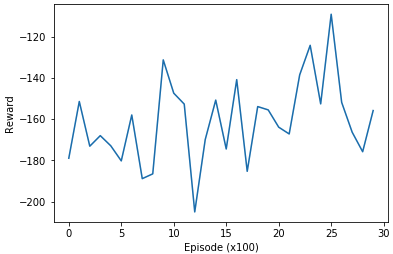
\includegraphics[width = \columnwidth]{sarsa_3k_alpha1}
  \caption{3000 episodes of SARSA with smoothing window of 100 episodes. Learning rate $\alpha = 0.1$, $\epsilon$-greedy policy selection with annealing steps from 1 to 0 over 2500 episodes.}
\label{alpha1}

  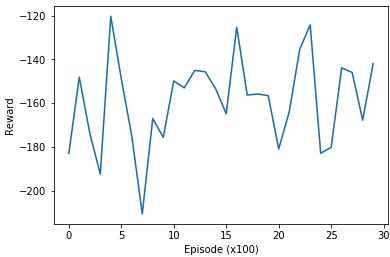
\includegraphics[width = \columnwidth]{sarsa_3k_alpha2}
  \caption{3000 episodes of SARSA with smoothing window of 100 episodes. Learning rate $\alpha = 0.2$, $\epsilon$-greedy policy selection with annealing steps from 1 to 0 over 2500 episodes.}
\label{alpha2}
\end{figure}


\begin{figure}[h]
  \includegraphics[width = \columnwidth]{sarsa_120k_01alpha}
  \caption{120000 episodes of SARSA with smoothing window of 3000 episodes. Learning rate $\alpha = 0.01$, $\epsilon$-greedy policy selection with annealing steps from 1 to 0 over 100000 episodes. }
\label{100ksmalleralpha}

  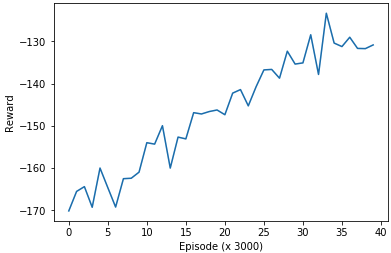
\includegraphics[width = \columnwidth]{sarsa_120k_3kwindow}
  \caption{120000 episodes of SARSA with smoothing window of 3000 episodes. Learning rate $\alpha = 0.1$, $\epsilon$-greedy policy selection with annealing steps from 1 to 0 over 100000 episodes. }
\label{100k}
\end{figure}



\subsection{Deep Q-Learning}

\begin{figure*}[h]
  \centering
  \includegraphics[width = 0.8 \textwidth]{Report/dqn_rewards.png}
  \caption{Average reward over 1000 episodes of DQN training with a smoothing window of 10 episodes. Learning rate was set to 0.0001, and a skip-frame parameter of 4 was used.}
  \label{dqn_rew}
\end{figure*}

When dealing with the DQN implementation, an important element to consider is the time needed for the training phase. Not having local access to graphical processing units capable of speeding up the learning process, we ended up taking advantage of Google's Colab\footnote{\url{https://colab.research.google.com/}} infrastructure. This Jupyter Notebook based system allows users to freely access a Nvidia Tesla K80 with 2496 CUDA cores and 12GB GDDR5 VRAM hosted on Google's cloud, for time limited sessions. Unfortunately the system is still in development and not completely stable, and we were unable to run the training for long sessions.

The network model we employed was sequential, with two convolutional and max-pooling steps, followed by three dense layers of decreasing size. The last layer only contained three nodes, as the number of available actions. We did notice a large impact due to the activation function chosen for the last dense layer. We originally selected to use a ReLu (rectified linear unit) on all our dense layers, but it caused the network to actually learn a deeply wrong policy, where the agent would always select the action \verb|move left|.

The main parameters we experimented with were:
\begin{itemize}
    \item learning rate;
    \item batch size;
    \item number of pre-train steps;
    \item discount rate.
\end{itemize}

We run all our experiments for a number of episodes varying between 1000 and 3000, depending on the availability of the infrastructure.
We did not find any particular improvement in varying the batch size (between 32 and 64 samples) and the discount rate (from 0.9 to 0.99) and we settled with a final value of 64 and 0.95 respectively. Similarly, we noticed that increasing the skip-frame parameter of the emulator, that is the number of frames on which the previously selected action is repeated before a new frame is presented to the agent, did not impact much the average reward, but it noticeably increased the training speed. Therefore, we set the skip-frame parameter to 4.

The best results, shown in \cref{dqn_rew}, were obtained with a learning rate of 0.0001, 5000 pre-training steps, a memory capacity of 10000, and updating the target network weights every 50 iterations. The results we obtained with the DQN, unfortunately, are non-conclusive, and we were probably limited by the scarce access to computational resources.



\section{Conclusion}
During this project we experimented with different variations on the main parameters of two famous Reinforcement Learning algorithms applied to the context of a first-person-shooter game. The average returns obtained by the agents were relatively low. This result was expected for the SARSA trained agent, as the algorithm is less suited for this kind of application.

The results from the deep-Q learning trained agent were non-conclusive. However, we do expect that, given enough time and computational resources for the training phase, the DQN agent should outperform the SARSA agent, as the algorithm has a history of success when applied to complex visual games. 

\medskip
\printbibliography

\end{document}